% Generated by extension/cross_study/make_assets.py. Do not edit.
\definecolor{donorcol}{HTML}{5D6670}
\definecolor{haocol}{HTML}{217D91}
\definecolor{coloncol}{HTML}{A64442}
\definecolor{betweencol}{HTML}{217D91}
\definecolor{withincol}{HTML}{C9803A}
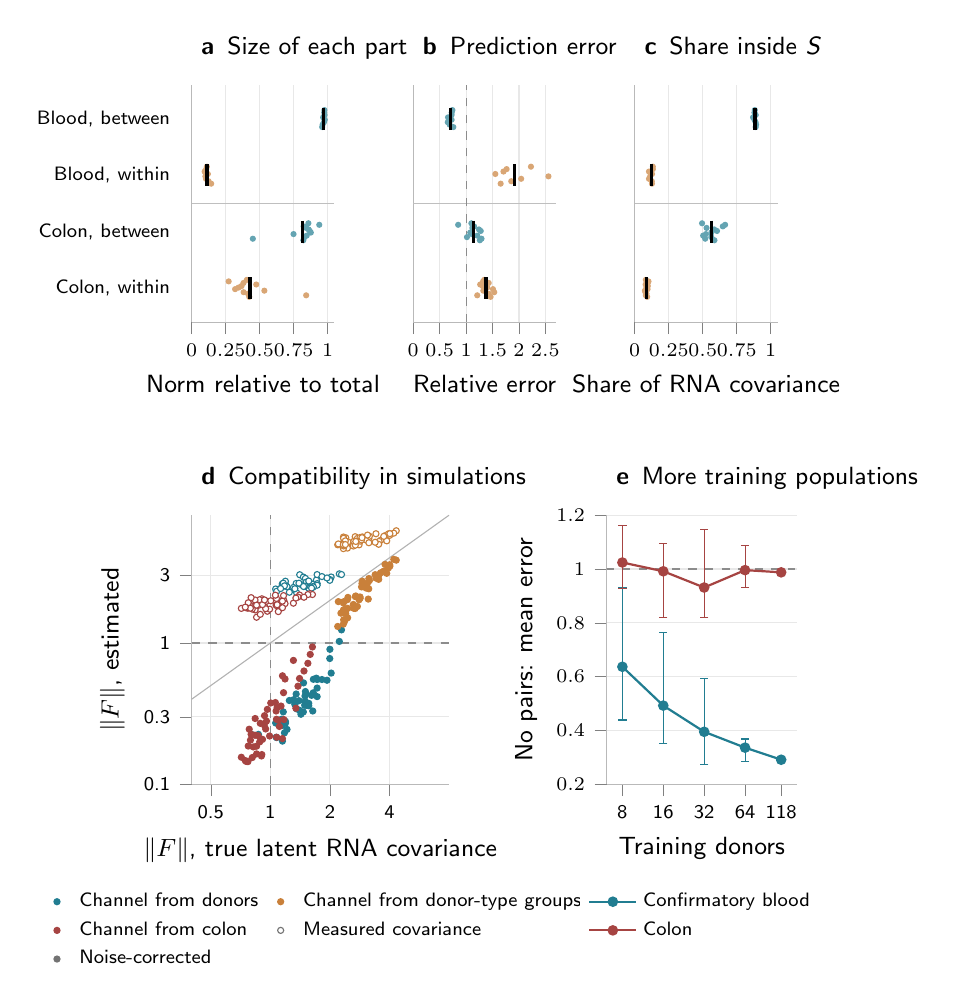
\begin{tikzpicture}[font=\sffamily]
\begin{axis}[name=pa,width=.28\textwidth,height=4.6cm,xmin=0,xmax=1.05,ymin=.4,ymax=4.6,
 xtick={0,.25,.5,.75,1},ytick={1,2,3,4},yticklabels={{Colon, within},{Colon, between},{Blood, within},{Blood, between}},xlabel={Norm relative to total},title={\textbf{a}\enspace Size of each part},
 axis x line*=bottom,axis y line*=left,tick align=outside,y tick style={draw=none},xmajorgrids=true,grid style={gray!18},axis line style={gray!55},tick label style={font=\sffamily\scriptsize},label style={font=\sffamily\small},clip=false,title style={font=\sffamily\small,at={(0,1)},anchor=base west,yshift=5pt}]
\draw[black!25] (axis cs:0,2.5) -- (axis cs:1.05,2.5);
\addplot[only marks,mark=*,mark size=.9pt,color=withincol!70] coordinates { (0.4233,0.850) (0.8419,0.877) (0.4147,0.905) (0.3821,0.932) (0.5345,0.959) (0.3194,0.986) (0.3447,1.014) (0.3670,1.041) (0.4749,1.068) (0.3810,1.095) (0.2721,1.123) (0.4058,1.150) };
\addplot[only marks,mark=|,mark size=4pt,line width=1.2pt,color=black] coordinates { (0.4301,1) };
\addplot[only marks,mark=*,mark size=.9pt,color=betweencol!70] coordinates { (0.8211,1.850) (0.4498,1.877) (0.8296,1.905) (0.8458,1.932) (0.7491,1.959) (0.8763,1.986) (0.8686,2.014) (0.8598,2.041) (0.8419,2.068) (0.8234,2.095) (0.9382,2.123) (0.8584,2.150) };
\addplot[only marks,mark=|,mark size=4pt,line width=1.2pt,color=black] coordinates { (0.8135,2) };
\addplot[only marks,mark=*,mark size=.9pt,color=withincol!70] coordinates { (0.1436,2.850) (0.1240,2.893) (0.1052,2.936) (0.1011,2.979) (0.1192,3.021) (0.0952,3.064) (0.1069,3.107) (0.1119,3.150) };
\addplot[only marks,mark=|,mark size=4pt,line width=1.2pt,color=black] coordinates { (0.1134,3) };
\addplot[only marks,mark=*,mark size=.9pt,color=betweencol!70] coordinates { (0.9596,3.850) (0.9627,3.893) (0.9728,3.936) (0.9790,3.979) (0.9666,4.021) (0.9772,4.064) (0.9747,4.107) (0.9762,4.150) };
\addplot[only marks,mark=|,mark size=4pt,line width=1.2pt,color=black] coordinates { (0.9711,4) };
\end{axis}
\begin{axis}[at={(pa.east)},anchor=west,xshift=1.0cm,name=pb,width=.28\textwidth,height=4.6cm,xmin=0,xmax=2.7,ymin=.4,ymax=4.6,
 xtick={0,.5,1,1.5,2,2.5},ytick={1,2,3,4},yticklabels={},xlabel={Relative error},title={\textbf{b}\enspace Prediction error},
 axis x line*=bottom,axis y line*=left,tick align=outside,y tick style={draw=none},xmajorgrids=true,grid style={gray!18},axis line style={gray!55},tick label style={font=\sffamily\scriptsize},label style={font=\sffamily\small},clip=false,title style={font=\sffamily\small,at={(0,1)},anchor=base west,yshift=5pt}]
\draw[black!25] (axis cs:0,2.5) -- (axis cs:2.7,2.5);
\draw[dashed,black!45] (axis cs:1,.4) -- (axis cs:1,4.6);
\addplot[only marks,mark=*,mark size=.9pt,color=withincol!70] coordinates { (1.4633,0.850) (1.2107,0.877) (1.4279,0.905) (1.5323,0.932) (1.3258,0.959) (1.5077,0.986) (1.3997,1.014) (1.3129,1.041) (1.2660,1.068) (1.4275,1.095) (1.3212,1.123) (1.3428,1.150) };
\addplot[only marks,mark=|,mark size=4pt,line width=1.2pt,color=black] coordinates { (1.3782,1) };
\addplot[only marks,mark=*,mark size=.9pt,color=betweencol!70] coordinates { (1.2597,1.850) (1.2915,1.877) (1.0163,1.905) (1.2113,1.932) (1.1092,1.959) (1.0779,1.986) (1.2769,2.014) (1.2425,2.041) (1.1182,2.068) (1.1504,2.095) (0.8499,2.123) (1.0999,2.150) };
\addplot[only marks,mark=|,mark size=4pt,line width=1.2pt,color=black] coordinates { (1.1420,2) };
\addplot[only marks,mark=*,mark size=.9pt,color=withincol!70] coordinates { (1.6535,2.850) (1.8537,2.893) (2.0413,2.936) (2.5572,2.979) (1.5532,3.021) (1.7068,3.064) (1.7664,3.107) (2.2263,3.150) };
\addplot[only marks,mark=|,mark size=4pt,line width=1.2pt,color=black] coordinates { (1.9198,3) };
\addplot[only marks,mark=*,mark size=.9pt,color=betweencol!70] coordinates { (0.7587,3.850) (0.6902,3.893) (0.6533,3.936) (0.7263,3.979) (0.6587,4.021) (0.7264,4.064) (0.7272,4.107) (0.7414,4.150) };
\addplot[only marks,mark=|,mark size=4pt,line width=1.2pt,color=black] coordinates { (0.7103,4) };
\end{axis}
\begin{axis}[at={(pb.east)},anchor=west,xshift=1.0cm,name=pc,width=.28\textwidth,height=4.6cm,xmin=0,xmax=1.05,ymin=.4,ymax=4.6,
 xtick={0,.25,.5,.75,1},ytick={1,2,3,4},yticklabels={},xlabel={Share of RNA covariance},title={\textbf{c}\enspace Share inside \textit{S}},
 axis x line*=bottom,axis y line*=left,tick align=outside,y tick style={draw=none},xmajorgrids=true,grid style={gray!18},axis line style={gray!55},tick label style={font=\sffamily\scriptsize},label style={font=\sffamily\small},clip=false,title style={font=\sffamily\small,at={(0,1)},anchor=base west,yshift=5pt}]
\draw[black!25] (axis cs:0,2.5) -- (axis cs:1.05,2.5);
\addplot[only marks,mark=*,mark size=.9pt,color=withincol!70] coordinates { (0.0914,0.850) (0.0816,0.877) (0.0859,0.905) (0.0785,0.932) (0.0750,0.959) (0.0943,0.986) (0.0855,1.014) (0.0961,1.041) (0.0800,1.068) (0.0953,1.095) (0.1011,1.123) (0.0814,1.150) };
\addplot[only marks,mark=|,mark size=4pt,line width=1.2pt,color=black] coordinates { (0.0872,1) };
\addplot[only marks,mark=*,mark size=.9pt,color=betweencol!70] coordinates { (0.5861,1.850) (0.5182,1.877) (0.5630,1.905) (0.5029,1.932) (0.5232,1.959) (0.5633,1.986) (0.6049,2.014) (0.5842,2.041) (0.5282,2.068) (0.6475,2.095) (0.6644,2.123) (0.4950,2.150) };
\addplot[only marks,mark=|,mark size=4pt,line width=1.2pt,color=black] coordinates { (0.5651,2) };
\addplot[only marks,mark=*,mark size=.9pt,color=withincol!70] coordinates { (0.1265,2.850) (0.1254,2.893) (0.1047,2.936) (0.1132,2.979) (0.1273,3.021) (0.1046,3.064) (0.1332,3.107) (0.1331,3.150) };
\addplot[only marks,mark=|,mark size=4pt,line width=1.2pt,color=black] coordinates { (0.1210,3) };
\addplot[only marks,mark=*,mark size=.9pt,color=betweencol!70] coordinates { (0.8893,3.850) (0.8923,3.893) (0.8886,3.936) (0.8801,3.979) (0.8700,4.021) (0.8897,4.064) (0.8801,4.107) (0.8826,4.150) };
\addplot[only marks,mark=|,mark size=4pt,line width=1.2pt,color=black] coordinates { (0.8841,4) };
\end{axis}
\begin{axis}[at={(pa.south west)},anchor=north west,yshift=-2.45cm,name=pd,
 width=.40\textwidth,height=5.0cm,xmode=log,ymode=log,xmin=.4,xmax=8,ymin=.1,ymax=8,
 xtick={.5,1,2,4},xticklabels={0.5,1,2,4},ytick={.1,.3,1,3},yticklabels={0.1,0.3,1,3},
 xlabel={$\|F\|$, true latent RNA covariance},ylabel={$\|F\|$, estimated},
 title={\textbf{d}\enspace Compatibility in simulations},
 axis x line*=bottom,axis y line*=left,tick align=outside,xmajorgrids=true,grid style={gray!18},axis line style={gray!55},tick label style={font=\sffamily\scriptsize},label style={font=\sffamily\small},clip=false,title style={font=\sffamily\small,at={(0,1)},anchor=base west,yshift=5pt},ymajorgrids=true,
 legend style={draw=none,font=\sffamily\scriptsize,at={(0.5,-0.36)},anchor=north,legend columns=2,column sep=5pt,cells={anchor=west}}]
\draw[dashed,black!45] (axis cs:1,.1) -- (axis cs:1,8);
\draw[dashed,black!45] (axis cs:.4,1) -- (axis cs:8,1);
\draw[black!30] (axis cs:.4,.4) -- (axis cs:8,8);
\addplot[only marks,mark=*,mark size=1.1pt,color=haocol,mark options={fill=white},forget plot] coordinates { (1.6380,2.6064) (1.1506,2.5665) (1.7078,2.7831) (1.4065,3.0374) (1.5154,2.5685) (1.1926,2.5968) (1.4678,2.9238) (1.1491,2.6169) (1.3573,2.2635) (1.0703,2.3409) (1.5034,2.8600) (1.1911,2.7323) (1.0634,2.4075) (0.8041,1.9401) (1.3253,2.4248) (1.1412,2.4816) (1.3500,2.6345) (1.1619,2.6481) (1.4989,2.5157) (1.2137,2.4963) (1.4908,2.5153) (1.1780,2.5331) (1.2471,2.2828) (1.0763,2.3185) (2.2305,3.0809) (1.7245,2.6276) (2.2885,3.0462) (2.0287,2.9261) (1.9995,2.8089) (1.6469,2.5100) (1.7230,3.0443) (1.4265,2.5920) (1.7234,2.5602) (1.5625,2.4347) (1.8226,2.9459) (1.5184,2.6935) (1.1263,2.4245) (0.8701,1.8791) (1.4956,2.5230) (1.3083,2.4676) (1.5632,2.7406) (1.3946,2.6457) (1.9966,2.7724) (1.6496,2.4909) (1.9331,2.8806) (1.6154,2.4431) (1.4711,2.5077) (1.3298,2.4162) };
\addplot[only marks,mark=*,mark size=1.1pt,color=haocol] coordinates { (1.6380,0.3303) (1.1506,0.2023) (1.7078,0.5636) (1.4065,0.3337) (1.5154,0.4366) (1.1926,0.2714) (1.4678,0.3254) (1.1491,0.2607) (1.3573,0.3419) (1.0703,0.2154) (1.5034,0.4534) (1.1911,0.2796) (1.0634,0.2718) (0.8041,0.2257) (1.3253,0.3809) (1.1412,0.2892) (1.3500,0.4355) (1.1619,0.3256) (1.4989,0.3876) (1.2137,0.2447) (1.4908,0.3633) (1.1780,0.2314) (1.2471,0.3918) (1.0763,0.2143) (2.2305,1.0252) (1.7245,0.5514) (2.2885,1.2374) (2.0287,0.6123) (1.9995,0.9016) (1.6469,0.4441) (1.7230,0.4798) (1.4265,0.3132) (1.7234,0.4175) (1.5625,0.3597) (1.8226,0.5512) (1.5184,0.3622) (1.1263,0.2799) (0.8701,0.2258) (1.4956,0.4219) (1.3083,0.3967) (1.5632,0.3742) (1.3946,0.3906) (1.9966,0.7762) (1.6496,0.5532) (1.9331,0.5449) (1.6154,0.4263) (1.4711,0.5220) (1.3298,0.3671) };
\addlegendentry{Channel from donors}
\addplot[only marks,mark=*,mark size=1.1pt,color=withincol,mark options={fill=white},forget plot] coordinates { (3.1244,5.5307) (2.3693,5.3944) (3.1419,5.4734) (2.6837,5.6422) (3.0481,5.3390) (2.4623,5.1231) (2.7522,5.4794) (2.4048,5.5432) (2.4524,4.6844) (2.2732,4.9906) (2.8399,5.5688) (2.3404,5.6081) (2.4570,5.1592) (2.1900,4.9439) (2.3392,4.6427) (2.2058,5.0129) (2.4658,5.1845) (2.3441,5.4966) (2.8088,4.9408) (2.3462,4.8506) (2.8430,5.2463) (2.3930,5.2694) (2.6257,4.8455) (2.3377,4.9592) (4.3282,6.2126) (3.7985,5.7286) (4.2058,5.9755) (3.9516,5.9057) (4.0093,5.7686) (3.6110,5.3154) (3.1665,5.6804) (2.9163,5.6201) (3.5205,5.0301) (3.5447,5.2217) (3.4173,5.9182) (3.0983,5.7902) (2.6410,5.2272) (2.3940,4.9632) (2.6884,4.9120) (2.7018,5.2184) (2.8899,5.3518) (2.9047,5.5469) (3.8739,5.2710) (3.5268,4.9844) (4.0196,5.9274) (3.7431,5.6698) (3.3859,5.1526) (3.1469,5.1112) };
\addplot[only marks,mark=*,mark size=1.1pt,color=withincol] coordinates { (3.1244,2.0429) (2.3693,1.4177) (3.1419,2.4147) (2.6837,1.7531) (3.0481,2.4429) (2.4623,1.7568) (2.7522,1.8118) (2.4048,1.6092) (2.4524,2.0241) (2.2732,1.6242) (2.8399,2.1139) (2.3404,1.7132) (2.4570,1.5058) (2.1900,1.3081) (2.3392,1.9196) (2.2058,1.9606) (2.4658,2.0992) (2.3441,1.9558) (2.8088,2.0193) (2.3462,1.4569) (2.8430,2.0712) (2.3930,1.7354) (2.6257,1.8713) (2.3377,1.3587) (4.3282,3.8511) (3.7985,3.5940) (4.2058,3.9028) (3.9516,3.3904) (4.0093,3.5725) (3.6110,3.1347) (3.1665,2.7621) (2.9163,2.7318) (3.5205,2.8373) (3.5447,3.0486) (3.4173,2.8763) (3.0983,2.6498) (2.6410,1.7579) (2.3940,1.6589) (2.6884,2.1258) (2.7018,2.1484) (2.8899,2.4899) (2.9047,2.6367) (3.8739,3.1068) (3.5268,2.8184) (4.0196,3.4933) (3.7431,3.2197) (3.3859,3.0379) (3.1469,2.8528) };
\addlegendentry{Channel from donor-type groups}
\addplot[only marks,mark=*,mark size=1.1pt,color=coloncol,mark options={fill=white},forget plot] coordinates { (1.1700,1.9941) (0.9010,1.9764) (1.1101,1.9394) (0.9054,2.0520) (1.0687,1.8537) (0.8827,2.0205) (0.9316,1.8408) (0.8364,2.0130) (0.8515,1.5195) (0.7703,1.7602) (0.9556,1.9725) (0.7991,2.0903) (0.8193,1.8077) (0.7134,1.7556) (0.8376,1.7129) (0.7818,1.8807) (0.8675,1.8420) (0.7729,1.9244) (0.9654,1.6752) (0.8099,1.7360) (0.9911,1.7334) (0.7550,1.7730) (0.8892,1.5931) (0.7929,1.7611) (1.5903,2.2306) (1.4043,2.1815) (1.6314,2.2007) (1.5471,2.1982) (1.4786,2.1054) (1.3792,2.1119) (1.1318,1.9790) (1.0733,2.0633) (1.0967,1.6658) (1.0755,1.8375) (1.1655,2.1615) (1.0599,2.1765) (0.8515,1.8498) (0.7464,1.7920) (0.9465,1.7473) (0.9123,1.8669) (1.0045,1.9873) (0.9342,2.0145) (1.3073,1.9106) (1.1862,1.8973) (1.3453,2.0770) (1.1505,1.9754) (1.1511,1.7755) (1.0817,1.8621) };
\addplot[only marks,mark=*,mark size=1.1pt,color=coloncol] coordinates { (1.1700,0.2871) (0.9010,0.1588) (1.1101,0.2568) (0.9054,0.1625) (1.0687,0.3303) (0.8827,0.1997) (0.9316,0.2628) (0.8364,0.2226) (0.8515,0.1863) (0.7703,0.1449) (0.9556,0.2802) (0.7991,0.2261) (0.8193,0.1840) (0.7134,0.1556) (0.8376,0.2923) (0.7818,0.2455) (0.8675,0.2207) (0.7729,0.1867) (0.9654,0.3392) (0.8099,0.1548) (0.9911,0.2198) (0.7550,0.1453) (0.8892,0.2703) (0.7929,0.2054) (1.5903,0.8301) (1.4043,0.5609) (1.6314,0.9368) (1.5471,0.7179) (1.4786,0.6332) (1.3792,0.4947) (1.1318,0.3579) (1.0733,0.2886) (1.0967,0.2845) (1.0755,0.2154) (1.1655,0.4450) (1.0599,0.3790) (0.8515,0.1643) (0.7464,0.1474) (0.9465,0.2465) (0.9123,0.2081) (1.0045,0.3764) (0.9342,0.3060) (1.3073,0.7527) (1.1862,0.5562) (1.3453,0.3457) (1.1505,0.2109) (1.1511,0.5859) (1.0817,0.3506) };
\addlegendentry{Channel from colon}
\addlegendimage{only marks,mark=*,mark size=1.1pt,color=black!55,mark options={fill=white}}
\addlegendentry{Measured covariance}
\addlegendimage{only marks,mark=*,mark size=1.1pt,color=black!55}
\addlegendentry{Noise-corrected}
\end{axis}
\begin{axis}[at={(pd.east)},anchor=west,xshift=2.0cm,name=pe,
 width=.33\textwidth,height=5.0cm,xmode=log,log basis x=2,
 xtick={8,16,32,64,118},xticklabels={8,16,32,64,118},
 ymin=0.2,ymax=1.2,xlabel={Training donors},ylabel={No pairs: mean error},
 title={\textbf{e}\enspace More training populations},
 title style={font=\sffamily\small,at={(0,1)},anchor=base west,yshift=5pt},
 axis x line*=bottom,axis y line*=left,tick align=outside,
 ymajorgrids=true,grid style={gray!18},axis line style={gray!55},
 tick label style={font=\sffamily\scriptsize},label style={font=\sffamily\small},
 legend style={draw=none,font=\sffamily\scriptsize,at={(0.5,-0.36)},anchor=north,legend columns=1,cells={anchor=west}}]
\draw[dashed,black!45] (axis cs:6,1) -- (axis cs:150,1);
\addplot[color=haocol,mark=*,mark size=1.5pt,line width=.8pt,error bars/.cd,y dir=both,y explicit] coordinates { (8,0.6369) += (0,0.2951) -= (0,0.1975) (16,0.4927) += (0,0.2730) -= (0,0.1401) (32,0.3954) += (0,0.1964) -= (0,0.1213) (64,0.3365) += (0,0.0323) -= (0,0.0505) (118,0.2916) += (0,0.0000) -= (0,0.0000) };
\addlegendentry{Confirmatory blood}
\addplot[color=coloncol,mark=*,mark size=1.5pt,line width=.8pt,error bars/.cd,y dir=both,y explicit] coordinates { (8,1.0243) += (0,0.1363) -= (0,0.0964) (16,0.9917) += (0,0.1029) -= (0,0.1710) (32,0.9314) += (0,0.2152) -= (0,0.1100) (64,0.9960) += (0,0.0918) -= (0,0.0644) (118,0.9878) += (0,0.0000) -= (0,0.0000) };
\addlegendentry{Colon}
\end{axis}
\end{tikzpicture}
